\documentclass[11pt]{article}

\usepackage{nmrdoc}
\usepackage{siunitx}
\usepackage{bm}
\usepackage{tikz}

\sisetup{per-mode=symbol}
\DeclareSIUnit{\angstrom}{\text{\AA}}
\DeclareSIUnit{\ppm}{ppm}

\newcommand{\code}[1]{\texttt{#1}}
\setlength{\parindent}{0pt}
\setlength{\parskip}{0.42em}
\emergencystretch=2em

\begin{document}
\NmrTitle{Numerical Addendum: Biot--Savart Calculator}

At the numerical level, the calculator is a closed-form wire field, summed
over the polygonal Johnson--Bovey double loop. The surrounding work supplies the
ring geometry, selects which atom--ring pairs are evaluated, turns the magnetic
field into an outer-product shielding kernel, records local ring-frame
coordinates, and projects the result into the shared \(T_0/T_1/T_2\)
representation. The listings below are distilled from the source --- loops and
bookkeeping trimmed --- but the constants, guards, and arithmetic are the
implementation's.

\section{Ring geometry and acceptance}

\code{GeometryResult} fills \code{conf.ring\_geometries} before this calculator
runs. Each aromatic ring contributes ordered vertices \(\bm v_i\) in
\(\si{\angstrom}\), their mean centre \(\bm c\), a unit normal \(\bm n\), and a
mean centre-to-vertex radius. The normal is the least-variance direction from an
SVD of the centred vertices, with its sign chosen by
\((\bm v_1-\bm v_0)\times(\bm v_2-\bm v_0)\). The Haigh--Mallion numerical
addendum treats that fit in full; here the Biot--Savart code consumes the
geometry. The vertex order matters here too: edge \(i\) runs from \(\bm v_i\)
to \(\bm v_j\), with \(j=(i+1)\bmod n\).

\begin{codebox}
conf.ring_geometries[ri] =
    protein.RingAt(ri).ComputeGeometry(positions);

double ring_cutoff = cfg("ring_current_spatial_cutoff");  // 15 A
auto nearby_rings = spatial.RingsWithinRadius(atom_pos, ring_cutoff);

ctx.distance = (atom_pos - geom.center).norm();
ctx.source_extent = 2.0 * geom.radius;                    // ring diameter
ctx.atom_index = ai;
ctx.source_ring_index = ri;
if (!filters.AcceptAll(ctx)) continue;
\end{codebox}

The spatial index is a KD-tree over ring centres, queried at
\(\SI{15}{\angstrom}\). It only proposes candidates. The filters then reject
centre distances \(<\SI{0.1}{\angstrom}\), distances
\(\le 0.5\,\code{source\_extent}=\code{geom.radius}\), and atoms that are ring
vertices or covalently bonded to one. These are binary gates: a rejected pair
does not enter the field sum, and no accepted contribution is reweighted.

The grid-sampling methods use the same double-loop kernel without atom-topology
filters. A grid point is skipped when its centre distance is below
\(\SI{0.1}{\angstrom}\), strictly inside the mean ring radius, or greater than
\(\SI{15}{\angstrom}\).

\section{One straight segment}

\code{WireSegmentField} is the numerical core. It takes segment endpoints
\(\bm a,\bm b\), field point \(\bm r\), and current \(I\) in SI units, then
returns \(\bm B\) in tesla. With
\(\bm\ell=\bm b-\bm a\), \(\bm d_A=\bm r-\bm a\), and
\(\bm d_B=\bm r-\bm b\), the code evaluates, with
\(\code{BIOT\_SAVART\_PREFACTOR}=10^{-7}\),
\[
  \bm B =
  10^{-7}\, I\,
  \frac{\bm\ell\times\bm d_A}{|\bm\ell\times\bm d_A|^2}
  \left(
    \frac{\bm\ell\cdot\bm d_A}{|\bm d_A|}
    -\frac{\bm\ell\cdot\bm d_B}{|\bm d_B|}
  \right).
\]

The cross product is the field direction for this segment. It is perpendicular
to the plane containing the wire and the field point, so it points around the
wire axis rather than along it. Its length is
\(|\bm\ell|d_\perp\), where \(d_\perp\) is the perpendicular distance from
\(\bm r\) to the line through the segment. The denominator is therefore
\((|\bm\ell|d_\perp)^2\), the squared distance factor in the closed form.

The bracket is the finite-length part of the line integral. Each term is the
scalar projection of \(\bm\ell\) onto an endpoint sight line:
\(\bm\ell\cdot\bm d_A/|\bm d_A|=|\bm\ell|\cos\alpha_A\) at endpoint
\(\bm a\), and \(\bm\ell\cdot\bm d_B/|\bm d_B|=|\bm\ell|\cos\alpha_B\) at
\(\bm b\). Their difference is the endpoint-cosine difference that replaces
the integral along the straight segment.

\begin{codebox}
Vec3 dl = b_m - a_m;
Vec3 dA = r_m - a_m;
Vec3 dB = r_m - b_m;

double lenA = dA.norm(), lenB = dB.norm();
if (lenA < cfg("biot_savart_wire_endpoint_guard") ||
    lenB < cfg("biot_savart_wire_endpoint_guard")) return Vec3::Zero();

Vec3 cross = dl.cross(dA);
double crossSq = cross.squaredNorm();
if (crossSq < cfg("biot_savart_wire_axis_guard")) return Vec3::Zero();

double scale = BIOT_SAVART_PREFACTOR * I_A / crossSq;
double proj = dl.dot(dA) / lenA - dl.dot(dB) / lenB;
return scale * proj * cross;
\end{codebox}

The two guards are the two ways this closed form degenerates. The endpoint
guard is \(10^{-25}\,\si{\metre}\), compared with \(|\bm d_A|\) and
\(|\bm d_B|\); at an endpoint, one endpoint projection divides by zero. The
axis guard is \(10^{-70}\), compared with \(|\bm\ell\times\bm d_A|^2\) after
metre conversion; on the wire axis \(d_\perp=0\), so both the azimuthal
direction and the denominator vanish. In either case the segment returns
\(\bm0\), with no limiting extrapolation.

\section{The double polygon loop}

\code{JohnsonBoveyField} builds the ring current from the segment field above.
It makes two copies of the ring polygon, one at \(+d_t\bm n\) and one at
\(-d_t\bm n\), where \(d_t=\code{ring.JohnsonBoveyLobeOffset()}\). The configured
offsets are \(\SI{0.64}{\angstrom}\) for PHE, TYR, and TRP6,
\(\SI{0.52}{\angstrom}\) for TRP5, \(\SI{0.50}{\angstrom}\) for HIS, HID, and
HIE, and \(\SI{0.60}{\angstrom}\) for TRP9. If the vertex count is below three,
the function returns \(\bm0\).

\begin{codebox}
int n = static_cast<int>(vertices.size());
if (n < 3) return Vec3::Zero();

Vec3 offset_ang = normal * lobe_offset_ang;
double halfI_A = 0.5 * current_nA * NANOAMPERES_TO_AMPERES;
Vec3 r_m = point_ang * ANGSTROMS_TO_METRES;

for (int i = 0; i < n; ++i) {
    int j = (i + 1) % n;
    Vec3 au = (vertices[i] + offset_ang) * ANGSTROMS_TO_METRES;
    Vec3 bu = (vertices[j] + offset_ang) * ANGSTROMS_TO_METRES;
    Vec3 al = (vertices[i] - offset_ang) * ANGSTROMS_TO_METRES;
    Vec3 bl = (vertices[j] - offset_ang) * ANGSTROMS_TO_METRES;
    B += WireSegmentField(au, bu, halfI_A, r_m);
    B += WireSegmentField(al, bl, halfI_A, r_m);
}
\end{codebox}

Each lobe carries half the requested current, so the current conversion
\(10^{-9}\,\si{\ampere}/\si{\nano\ampere}\) happens once in
\code{halfI\_A}. Positions cross the boundary once as well:
\(10^{-10}\,\si{\metre}/\si{\angstrom}\) is applied to the field point and to
each segment endpoint. After those conversions, \code{WireSegmentField} sees
only metres, amperes, and tesla. The \(10^6\) ppm scale does not enter this
field calculation; it reappears when \(\bm B\) becomes a shielding kernel.

The loop is the polygon through the ring vertices. A five-, six-, or
nine-membered ring contributes five, six, or nine straight segments per lobe,
with the last edge wrapping to the first vertex. The segment formula is exact
for those straight chords. The approximation is the replacement of the smooth
ring-current path by that polygonal path, not a quadrature over the loop.

\begin{figure}[ht]
\centering
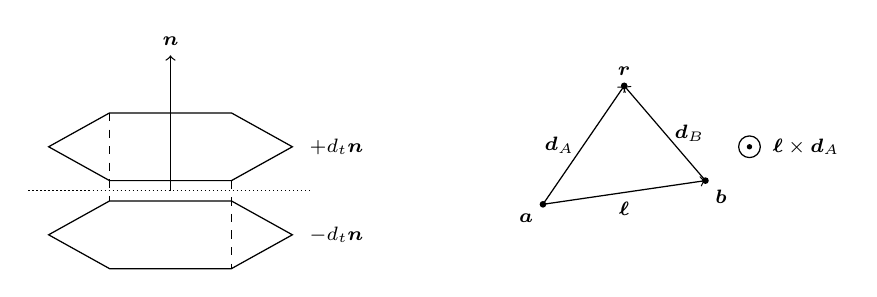
\begin{tikzpicture}[scale=0.86,line width=0.45pt]
  \coordinate (C) at (0,0);
  \coordinate (N) at (0,2.0);
  \coordinate (U1) at (-1.8,0.65);
  \coordinate (U2) at (-0.9,1.15);
  \coordinate (U3) at (0.9,1.15);
  \coordinate (U4) at (1.8,0.65);
  \coordinate (U5) at (0.9,0.15);
  \coordinate (U6) at (-0.9,0.15);
  \coordinate (L1) at (-1.8,-0.65);
  \coordinate (L2) at (-0.9,-0.15);
  \coordinate (L3) at (0.9,-0.15);
  \coordinate (L4) at (1.8,-0.65);
  \coordinate (L5) at (0.9,-1.15);
  \coordinate (L6) at (-0.9,-1.15);

  \draw[->] (C) -- (N) node[above] {\scriptsize \(\bm n\)};
  \draw[densely dotted] (-2.1,0) -- (2.1,0);
  \draw (U1)--(U2)--(U3)--(U4)--(U5)--(U6)--cycle;
  \draw (L1)--(L2)--(L3)--(L4)--(L5)--(L6)--cycle;
  \draw[dashed] (U2) -- (L2);
  \draw[dashed] (U5) -- (L5);
  \node at (2.45,0.65) {\scriptsize \(+d_t\bm n\)};
  \node at (2.45,-0.65) {\scriptsize \(-d_t\bm n\)};

  \begin{scope}[xshift=5.5cm,yshift=-0.2cm]
    \coordinate (A) at (0,0);
    \coordinate (B) at (2.4,0.35);
    \coordinate (R) at (1.2,1.75);
    \draw[->] (A) -- (B) node[midway,below] {\scriptsize \(\bm\ell\)};
    \draw[->] (A) -- (R) node[midway,left] {\scriptsize \(\bm d_A\)};
    \draw[->] (B) -- (R) node[midway,right] {\scriptsize \(\bm d_B\)};
    \fill (A) circle (1.4pt) node[below left] {\scriptsize \(\bm a\)};
    \fill (B) circle (1.4pt) node[below right] {\scriptsize \(\bm b\)};
    \fill (R) circle (1.4pt) node[above] {\scriptsize \(\bm r\)};
    \draw (3.05,0.85) circle (0.16);
    \fill (3.05,0.85) circle (0.04);
    \node[right] at (3.25,0.85) {\scriptsize \(\bm\ell\times\bm d_A\)};
  \end{scope}
\end{tikzpicture}
\caption{The Johnson--Bovey field is the sum of straight-wire fields over two
offset polygons. One segment uses \(\bm\ell=\bm b-\bm a\) and endpoint vectors
\(\bm d_A,\bm d_B\); \(\bm\ell\times\bm d_A\) points in the segment's azimuthal
field direction.}
\end{figure}

\section{The shielding kernel}

For atom calculations the double-loop field is always called with
\code{current\_nA = 1.0}. The code records \code{ring.Intensity()} for
provenance, but \code{Compute()} does not multiply by it. This unit-current
convention separates the geometric kernel from the fitted or literature
ring-current intensity: \(\bm B\) is the field of a \(\SI{1}{\nano\ampere}\)
Johnson--Bovey loop at the accepted atom position.

\[
  G_{ab} = -\,n_b B_a\,\code{PPM\_FACTOR},
  \qquad \code{PPM\_FACTOR}=10^6 .
\]

\begin{codebox}
Vec3 B = JohnsonBoveyField(geom.vertices, geom.normal,
                           ring.JohnsonBoveyLobeOffset(), 1.0, atom_pos);

Mat3 G;
for (int a = 0; a < 3; ++a)
    for (int b = 0; b < 3; ++b)
        G(a,b) = -geom.normal(b) * B(a) * PPM_FACTOR;

rn->G_tensor = G;
rn->G_spherical = SphericalTensor::Decompose(G);
rn->B_field = B;
G_total += G;
B_total += B;
\end{codebox}

The row index \(a\) is the secondary-field component, and the column index
\(b\) is the applied-field component. The matrix is the outer product
\(-\bm B\bm n^{\mathsf T}\), scaled by \(10^6\), so its rank is at most one.
It is generally asymmetric because \(\bm B\) need not be parallel to
\(\bm n\). The trace is \(-10^6\,\bm n\cdot\bm B\), hence
\(T_0=-10^6(\bm n\cdot\bm B)/3\), while the antisymmetric and symmetric
traceless parts can also be populated.

\code{WriteFeatures()} exports the per-atom fields \code{Compute()} wrote.
\code{bs\_shielding.npy} is \((N,9)\), the decomposition of \(G\) summed over all
rings at the atom, packed in \(T_0,T_1,T_2\) order. The per-type arrays
\code{bs\_per\_type\_T0.npy} and \code{bs\_per\_type\_T2.npy} are \((N,8)\) and
\((N,40)\), eight aromatic ring-type slots carrying one \(T_0\) and five \(T_2\)
components each. The remaining two are \code{bs\_total\_B.npy} at \((N,3)\) and
\code{bs\_ring\_counts.npy} at \((N,4)\) for the \(\le3,\le5,\le8,\le12\)
\(\si{\angstrom}\) shells. The per-type accumulation stores
\(T_0\) and \(T_2\) only; the full \((N,9)\) channel keeps \(T_1\).

\section{The ring-frame record}

The ring calculators share \code{RingNeighbourhood} records. When this
calculator creates the record for an accepted atom--ring pair, it stores a local
ring-frame description before writing the Biot--Savart fields. With
\(\bm d=\bm r-\bm c\), the axial coordinate is \(z=\bm d\cdot\bm n\), the
in-plane vector is \(\bm d_\perp=\bm d-z\bm n\), its length is
\(\rho=|\bm d_\perp|\), and the folded polar angle is
\(\theta=\operatorname{atan2}(\rho, |z|)\). The fold makes \(\theta\) the same
above and below the ring; \(z\) keeps the side sign.

\begin{codebox}
Vec3 d = atom_pos - geom.center;
double z = d.dot(geom.normal);
Vec3 d_plane = d - z * geom.normal;
double rho = d_plane.norm();
double theta = std::atan2(rho, std::abs(z));

Vec3 ref = geom.vertices[0] - geom.center;
Vec3 ref_plane = ref - ref.dot(geom.normal) * geom.normal;
double ref_norm = ref_plane.norm();
double rho_guard = cfg("near_zero_vector_norm_threshold");  // 1e-10

if (rho > rho_guard && ref_norm > rho_guard) {
    Vec3 d_hat = d_plane / rho;
    Vec3 ref_hat = ref_plane / ref_norm;
    rn->cos_phi = d_hat.dot(ref_hat);
    rn->sin_phi = d_hat.cross(ref_hat).dot(geom.normal);
}
\end{codebox}

The azimuth reference is the projected centre-to-vertex-zero direction. The
stored cosine gives the cosine of the opening angle between that reference and
the atom's in-plane direction, but the cosine alone cannot distinguish the two
sides of that reference line. The stored sine,
\((\hat{\bm d}_\perp\times\hat{\bm r}_0)\cdot\bm n\), changes sign across that
line under the oriented ring normal. That sign distinguishes the two in-plane
sides of an asymmetric ring, such as the nitrogen side and carbon side of an
imidazole. If either in-plane vector has norm at most \(10^{-10}\), the
normalization is skipped and the default
\((\code{cos\_phi},\code{sin\_phi})=(1,0)\) remains.

The magnetic field is projected into the same frame. The radial unit vector is
formed only when \(\rho>10^{-10}\); otherwise it is left at \(\bm0\). The stored
\code{B\_cylindrical} vector is
\((B_\rho,0,B_z)=(\bm B\cdot\hat{\bm\rho},0,\bm B\cdot\bm n)\). The azimuthal
field component is not stored in this summary.

\section{The shared tensor projection}

Every \(3\times3\) tensor emitted by this calculator passes through
\code{SphericalTensor::Decompose}. The projection is closed-form arithmetic,
not an eigenproblem: the trace gives \(T_0\), the antisymmetric part gives the
three \(T_1\) components, and the symmetric traceless part gives the five
\(T_2\) components.

\begin{codebox}
st.T0 = sigma.trace() / 3.0;

st.T1[0] = 0.5*(sigma(1,2) - sigma(2,1));
st.T1[1] = 0.5*(sigma(2,0) - sigma(0,2));
st.T1[2] = 0.5*(sigma(0,1) - sigma(1,0));

double Sxx = sigma(0,0) - st.T0;
double Syy = sigma(1,1) - st.T0;
double Szz = sigma(2,2) - st.T0;
double Sxy = 0.5*(sigma(0,1) + sigma(1,0));
double Sxz = 0.5*(sigma(0,2) + sigma(2,0));
double Syz = 0.5*(sigma(1,2) + sigma(2,1));

st.T2[0] = std::sqrt(2.0) * Sxy;
st.T2[1] = std::sqrt(2.0) * Syz;
st.T2[2] = std::sqrt(3.0 / 2.0) * Szz;
st.T2[3] = std::sqrt(2.0) * Sxz;
st.T2[4] = (Sxx - Syy) / std::sqrt(2.0);
\end{codebox}

The \(T_2\) packing is isometric: the five-vector length equals the Frobenius
length of the symmetric traceless matrix \(\bm S\). The off-diagonal
\(\sqrt2\) factors pay for double counting, since \(S_{xy}\) appears as both
\(S_{xy}\) and \(S_{yx}\) in the matrix. The diagonal pair
\(\sqrt{3/2}\,S_{zz}\) and \((S_{xx}-S_{yy})/\sqrt2\) carries the two remaining
degrees of freedom after \(S_{xx}+S_{yy}+S_{zz}=0\). A dot product of stored
\(T_2\) five-vectors is therefore the Frobenius inner product of the symmetric
traceless matrices they encode. For the Biot--Savart kernel, all three
channels can be populated because \(G=-10^6\bm B\bm n^{\mathsf T}\) is
generally asymmetric.

\section{Glossary}

\textbf{Finite-wire Biot--Savart field.} A straight current segment curls the
magnetic field around its axis, and the endpoint sight lines set how much of
that curl reaches the field point (an azimuthal field, scaled by a
finite-length factor). One edge of a six-membered ring is one
such segment; its \(\bm\ell\times\bm d_A\) fixes the azimuthal direction and its
two endpoint projection terms give the finite-length cosine difference.
Formally, it is the analytic line integral of
\(\mu_0 I\,d\bm\ell\times\bm R/(4\pi|\bm R|^3)\) over a straight segment; the
implementation uses \(10^{-7}\) for \(\mu_0/(4\pi)\).

\textbf{Johnson--Bovey double loop.} Two displaced copies of the ring polygon,
one above and one below the fitted ring plane, model the two off-plane
\(\pi\)-electron sheets. For a PHE ring those copies sit at
\(\pm\SI{0.64}{\angstrom}\,\bm n\), and each carries half of the requested
current. Formally, the field is the sum of the closed-form finite-wire field
over all polygon edges of both displaced loops.

\textbf{Rank-at-most-one outer product.} A column vector times a row vector can
change only along one input direction, and it becomes the zero matrix if either
vector is zero. Here \(G=-10^6\bm B\bm n^{\mathsf T}\), so a field component
\(B_a\) fills row \(a\) in proportion to the normal components \(n_b\).
Formally, \(\operatorname{rank}(\bm u\bm v^{\mathsf T})\le 1\) for all
\(\bm u,\bm v\).

\textbf{Spherical tensor decomposition, \(T_0/T_1/T_2\).} A \(3\times3\)
tensor holds three kinds of content that rotate without mixing --- an
orientation-free size (the scalar trace, \(T_0\)), an axial twist from its
antisymmetric part (the three \(T_1\) components), and a five-number traceless
shape for the rest of the direction-dependence (the five \(T_2\) components).
For one ring's kernel here \(T_0\) is
\(-10^6(\bm n\cdot\bm B)/3\), while \(T_1\) records the antisymmetry when
\(\bm B\) and \(\bm n\) are not parallel. Formally, it is the closed-form split
of a \(3\times3\) tensor's nine components into dimensions \(1\), \(3\), and
\(5\), with the \(T_2\) basis normalized to preserve the Frobenius norm.

\textbf{Ring-frame coordinates.} The atom position is split into height above
the ring and in-plane distance from the centre. A point over an imidazole's
nitrogen side and one over its carbon side can have the same \(\rho\) and \(z\),
but opposite stored signed azimuth. Formally, the frame stores
\((z,\rho,\theta,\cos\phi,\sin\phi)\) with \(z=\bm d\cdot\bm n\),
\(\rho=|\bm d-z\bm n|\), \(\cos\phi=\hat{\bm d}_\perp\cdot\hat{\bm r}_0\), and
\(\sin\phi=(\hat{\bm d}_\perp\times\hat{\bm r}_0)\cdot\bm n\).

\end{document}
